\documentclass[12pt]{article}

\usepackage{graphicx}
\usepackage{paralist}
\usepackage{listings}
\usepackage{booktabs}
\usepackage{hyperref}
\usepackage{subfig}
\usepackage{float}
\usepackage{mathtools}
\usepackage{fancyvrb}

\DeclarePairedDelimiter\ceil{\lceil}{\rceil}
\DeclarePairedDelimiter\floor{\lfloor}{\rfloor}
\oddsidemargin 0mm
\evensidemargin 0mm
\textwidth 160mm
\textheight 200mm

\pagestyle {plain}
\pagenumbering{arabic}

\newcounter{stepnum}

\title{CS/SE 2XB3 Lab 5 Report\\Enrolled in CSL02}
\author{
  Wang, Mingzhe\\400316660\\
  \texttt{wangm235@mcmaster.ca}
  \and
  Li, Xing\\400292346\\
  \texttt{li64@mcmaster.ca}
  \and
  Moon, Hyosik\\400295620\\
  \texttt{moonh8@mcmaster.ca}
  }
\date{\today}



\begin{document}
\bibliographystyle{plain}

\maketitle

\tableofcontents
\newpage

\section{Building Heaps}
\subsection{Estimation}
\begin{itemize}
\item build\_heap\_1 Bottom-up. Since each sink has worst case $O(\log n)$ and there are $n/2$ loops, the time complexity of "build\_heap\_1 Bottom-up" is $O(\frac {1}{2} n \log n) = O(n \log n)$.
\item build\_heap\_2 Brick-by-brick. As each insert has worst case $O(\log n)$ and there are n inserts, the time complexity of "build\_heap\_2 Brick-by-brick" is $O(n \log n)$.
% \item build\_heap\_3 Sink-top-down. As each sink has worst case $O(\log n)$ and Sink-top-down calls n sinks at least,  the time complexity of "build\_heap\_3 Sink-top-down" is at least $O(n \log n)$. However, as it cannot guarantee the result is heap. In the cases when the big values are all at the left of the heap tree and small values are all at the right of the heap tree, it may cause log n times "Sink-top-down". The figure \ref{Figure: build3_worst} below is an example. It takes 3 times to build a heap by sinking top-down. The time complexity of "build\_heap\_3 Sink-top-down" could be as bad as $O(n \log^2 n)$
% \end{itemize}
% \begin{figure}[hbt!]
%     \centering
%     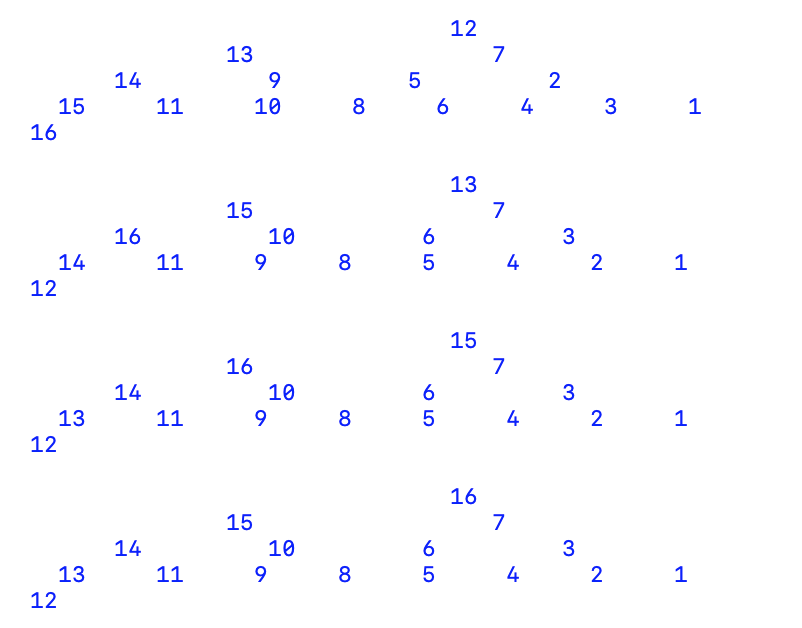
\includegraphics[width=0.5\textwidth]{Figures/build3_worst.png}
%     \caption{build heap 3 Sink-top-down: Worst Case}
%      \label{Figure: build3_worst}
% \end{figure}

\item build\_heap\_3 Sink-top-down. As each sink has worst case $O(\log n)$ and Sink-top-down calls n sinks at least,  the time complexity of "build\_heap\_3 Sink-top-down" is at least $O(n \log n)$. However, as it cannot guarantee the result is heap. When the biggest value is at the bottom of the heap, it should repeat the heap process until it goes to the top. Because each time it goes up just one level, it needs $\floor{log{n}}$ repetitions of the for-loop. Thus, the time complexity of "build\_heap\_3 Sink-top-down" could be as bad as $O(n \log^2 n)$.
\end{itemize}

\newpage
\subsection{Experiment Results. build\_heap\_1, build\_heap\_2}
In order to obtain the experimental data of Bottom\_up(heap1) and Brick\_by\_Brick(heap2)
, we tested them by increasing the number of elements 
from 100 to 20,000, step by 100. We ran them 5 times at each point and 
took the average runtimes. 

~\newline\noindent Different from what we expected, both of them showed
 $O(n)$ time complexities. This is because in the case of Bottom\_up(heap1),
 when we set the $h$ as the height of a heap(0 at the bottom), 
 and $n$ is the total number of elements of a heap, then it has the number of
 $ \ceil*{\frac{n}{2^{h+1}}} $ elements at each height. Because each element
 has at most $one$ swap, it showed that the time complexity of 
 $ \Sigma_{h=1}^{ \floor{log{n}}} \ceil*{\frac{n}{2^{h+1}}} * O(1)
  = O(n * \Sigma_{h=1}^{log{n}} \frac{1}{2^{h}}) = O(n)$.  
Similarly, in the case of Brick\_by\_Brick(heap2), each element 
has the time complexity of $O(h)$ at a height $h$. 
As a result, it showed the time complexity of $ \Sigma_{h=0}^{ \floor{log{n}}} 
\ceil*{\frac{n}{2^{h+1}}} * O(h) = O(n * \Sigma_{h=0}^{log{n}} \frac{h}{2^{h}}) 
= O(n * \Sigma_{h=0}^{\infty} \frac{h}{2^{h}}) = O(n)$. \cite{wikipedia}

\begin{figure}[hbt!]
  \centering
  \subfloat[Bottom\_up(build\_heap\_1)]{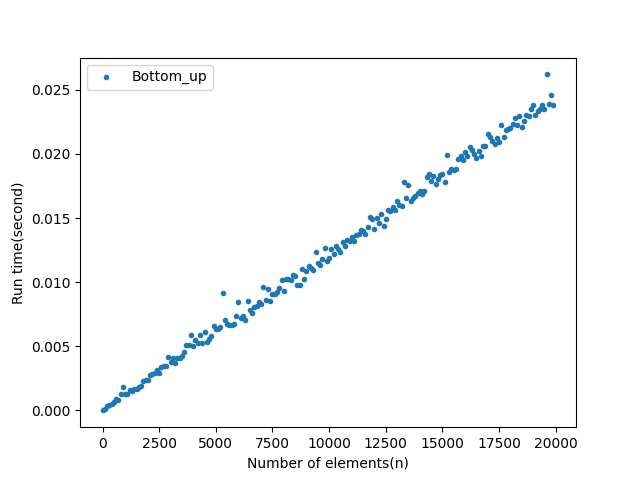
\includegraphics[width=0.49\textwidth]{Figures/Bottom_up.png}\label{r1}}
  \hfill
  \subfloat[Brick\_by\_Brick(build\_heap\_2)]{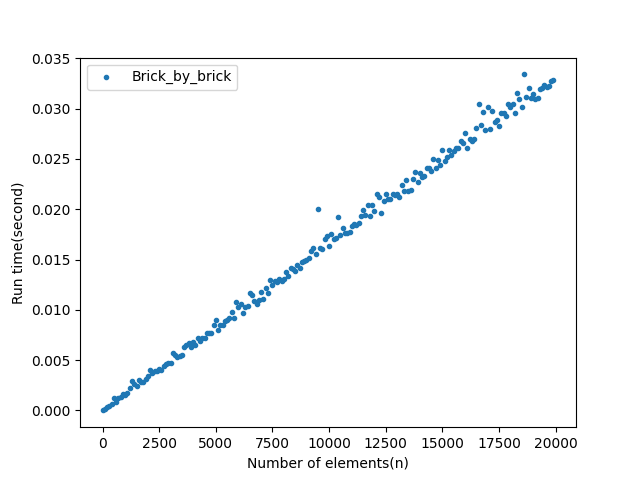
\includegraphics[width=0.49\textwidth]{Figures/Brick_by_brick.png}\label{r2}}
  \caption{Time complexities of heap1, heap2}
\end{figure}


\subsection{Experiment Results. build\_heap\_3}
We tested Sink\_top\_down(heap3) under the same test condition. 
As we expected, it showed the time complexity of $O(nlogn)$ ({Figure \ref{r3}, \ref{r4}}).
When we see the Figure \ref{r3}, it seems to be a leaner function but its runtime 
is longer than the previous heaps (heap1, heap2). When we divdie it $n$, it shows 
a logarithmic function. When we take log at each x, y value, then its slope is 
about $1.128$ which means it's not an exact linear function (Figure \ref{r5}).

\begin{figure}[hbt!]
  \centering
  \subfloat[Sink\_top\_down(heap3)]{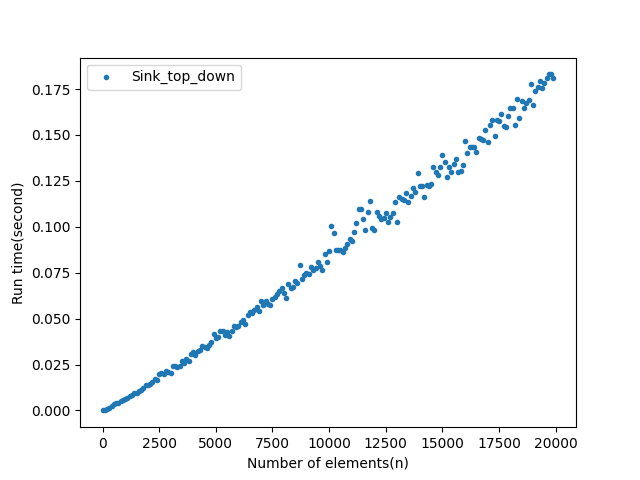
\includegraphics[width=0.49\textwidth]{Figures/Sink_top_down.png}\label{r3}}
  \hfill
  \subfloat[Runtime / n]{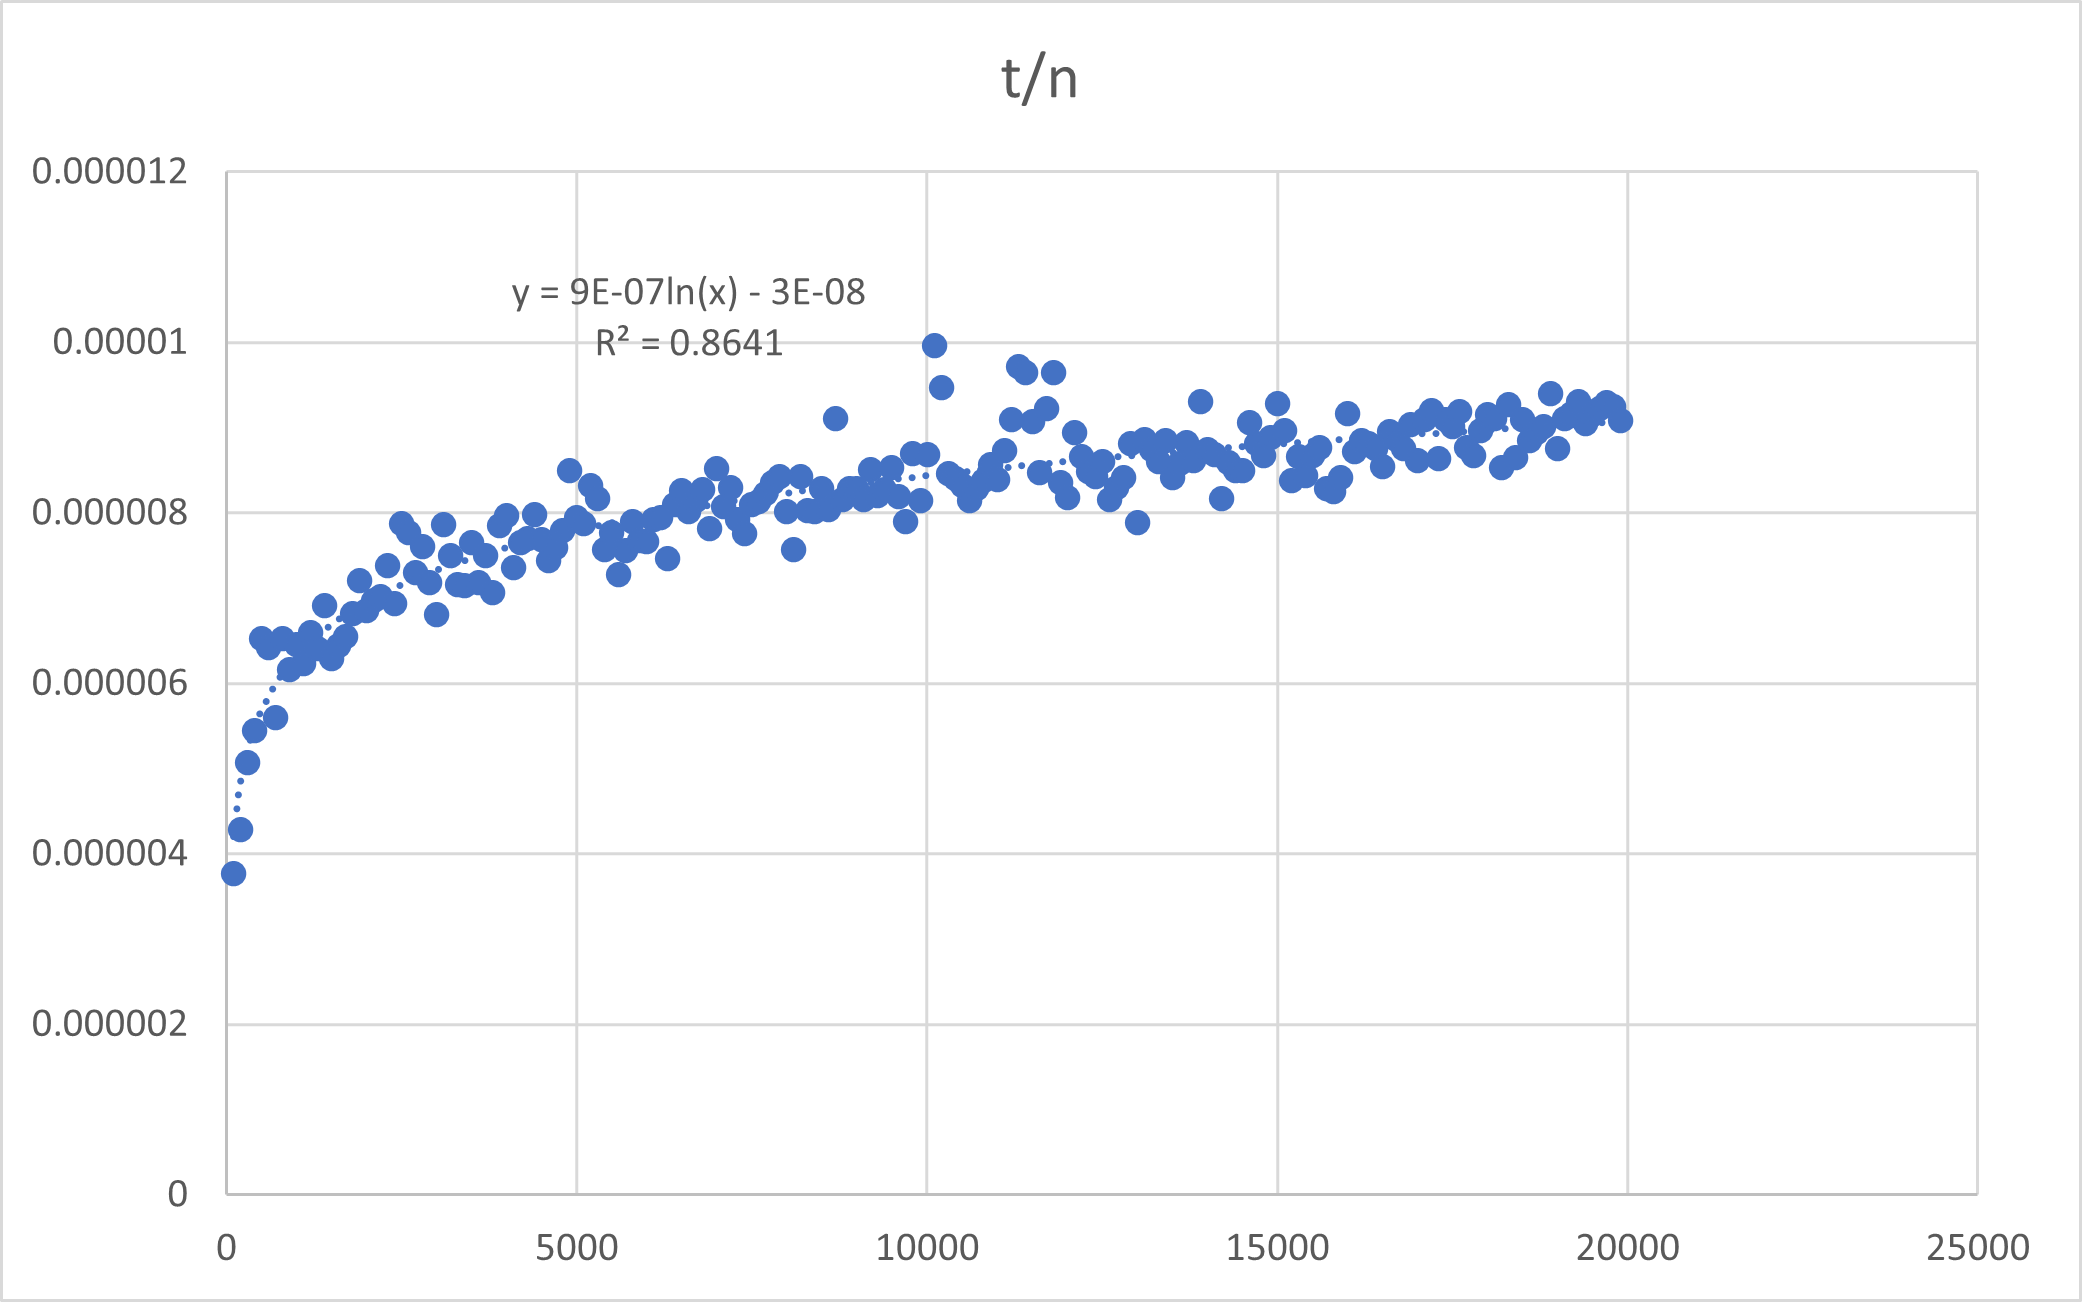
\includegraphics[width=0.49\textwidth]{Figures/Sink_top_down2.png}\label{r4}}
  \caption{Time complexity of heap3}
\end{figure}

\begin{figure}[hbt!]
  \centering
  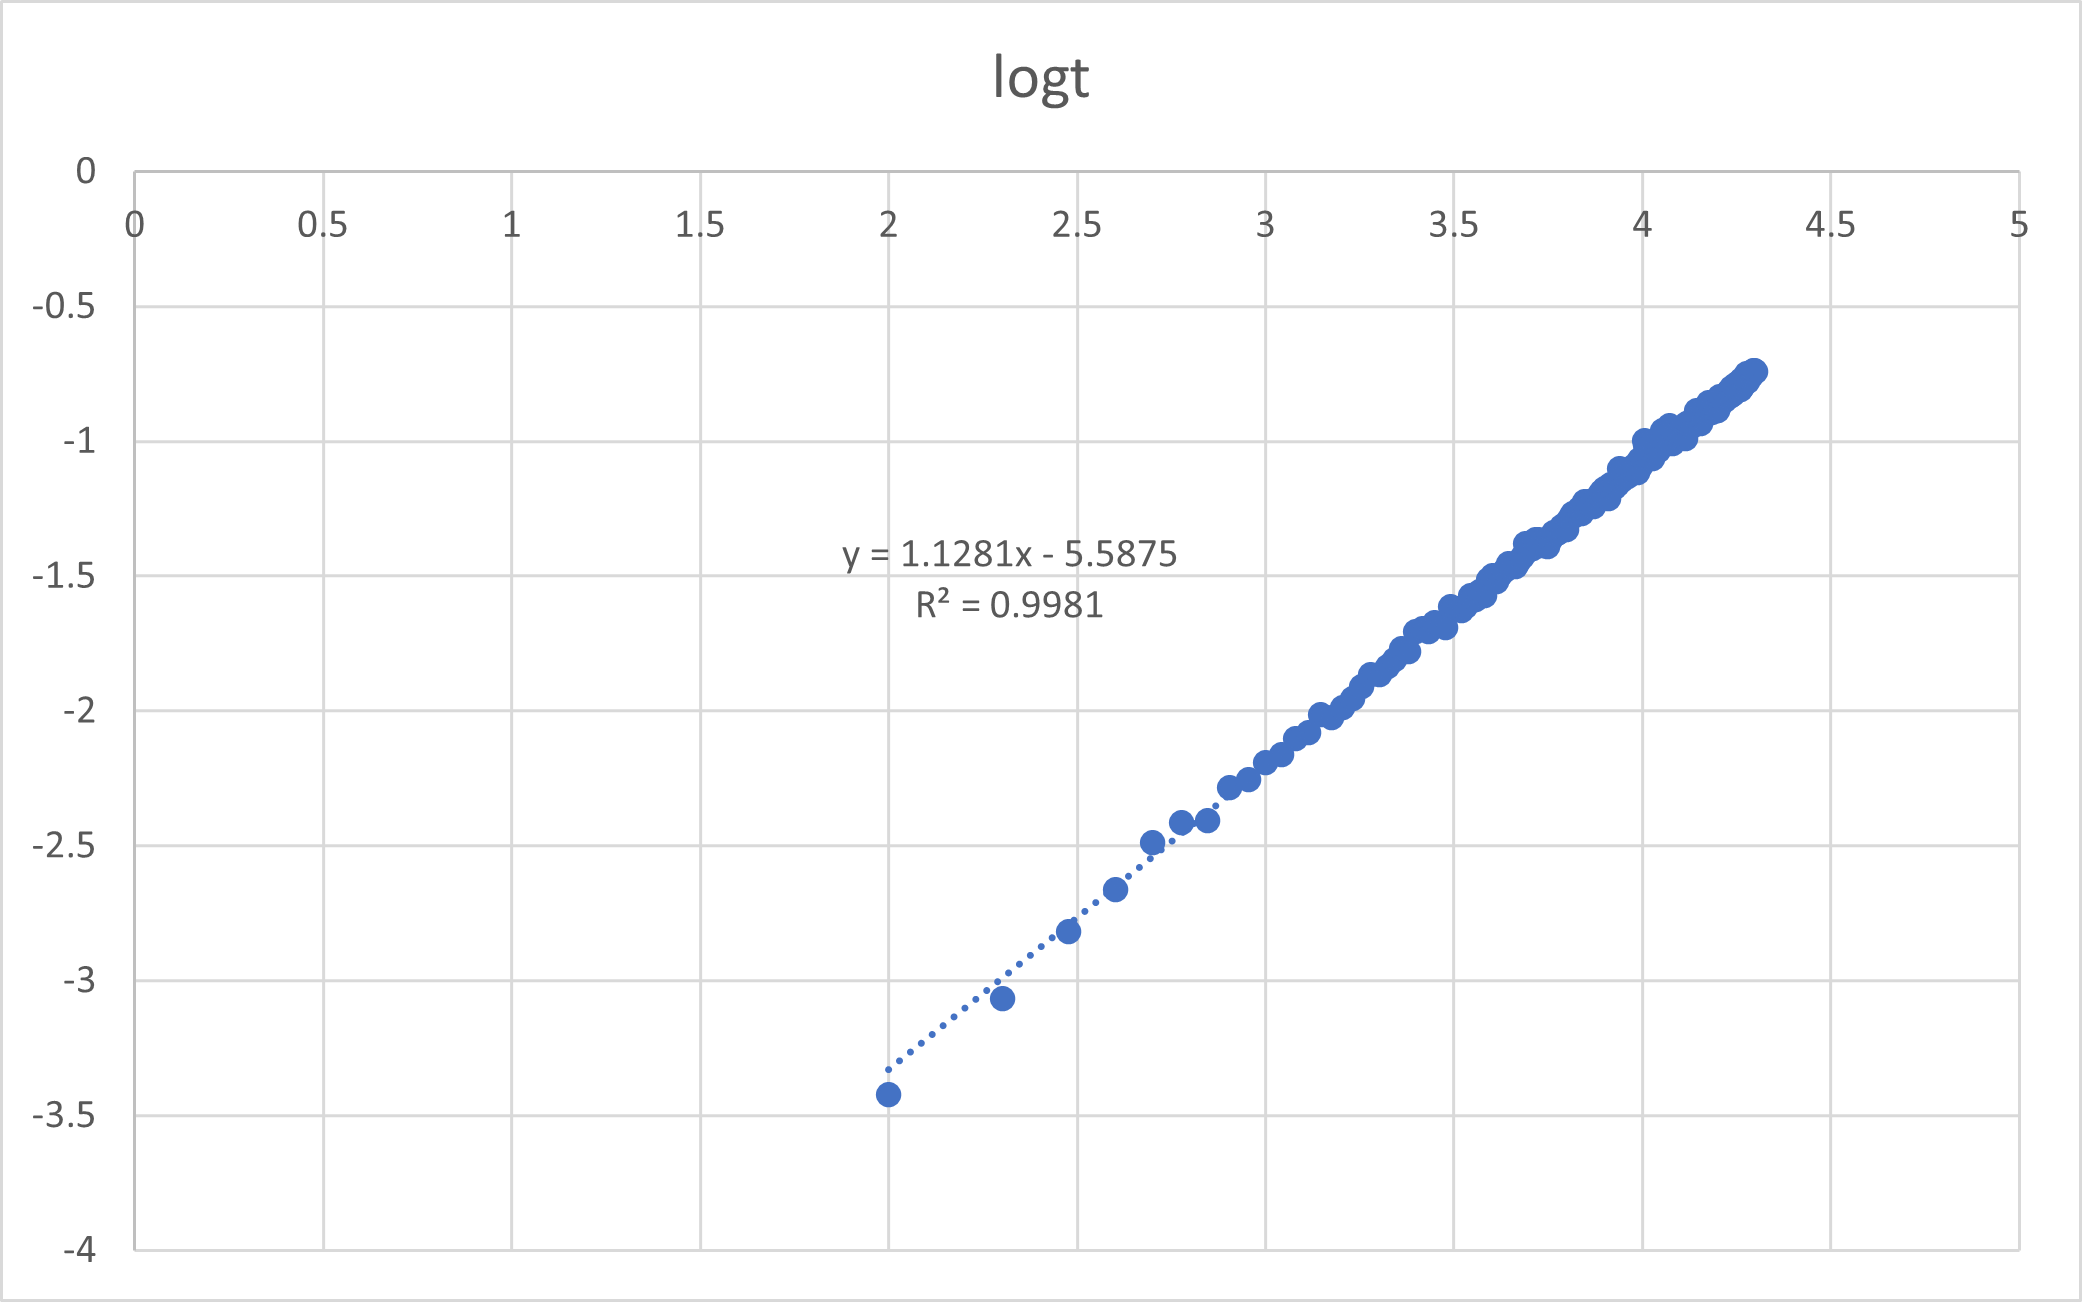
\includegraphics[width=0.5\textwidth]{Figures/Sink_top_down3.png}
  \caption{Time complexity of heap3 (log)}
   \label{r5}
\end{figure}

\newpage
% \subsection{What Causes Poor Performance of build\_heap\_3?}
% The poor performance of build\_heap\_3 is caused by the heapifying order. In comparison with build\_heap\_1, the only difference is bottom-up vs top-down. This is because with bottom-up heapifying,  the maximum number of times we need to heapify every node is 1. When each node is sinked in the bottom-up order, we can know that the substree of this node is already heapified. After recursively do the sinking, no additional heapifying is required. On the contrary, when the node is sinked in the top-down order, the whole array is heapish at different levels while different micro heapish structure may conflict with each other. The way to improve is to change the heaifying order.
\subsection{What Causes Poor Performance of build\_heap\_3?}
For build\_heap\_3, an element of the implementation that causes poor performance is that at the end of each iteration of heapifying every node, it needs to check if the result structure is a heap by calling \verb|is_heap|. However, \verb|is_heap| itself is a function that needs $O(n)$ complexity. Thus, this behavior will induce poor performance of build\_heap\_3.

~\newline\noindent
As the hint remind us, we notice that the maximum number of times you need to heapify every node before the whole thing is a heap should be no lager than the complete binary tree (heap)'s height. Thus, we find a improvement that at the end of each iteration of heapifying every node we do not perform \verb|is_heap| check anymore, instead we simply set the number of times of heapifying every node to be the heap's height for all the cases. By doing this, we abandon the \verb|is_heap|'s complexity $O(n)$ in the inner loop, which could improve the implementation. 

~\newline\noindent
Note:
\begin{itemize}
\item The improved implementation can be found in the \verb|heap.py| named \verb|build_heap3_opt|.
\item For calculating the complete binary tree (heap)'s height by its number of nodes. The function we used is as the following:
\begin{lstlisting}
math.ceil(math.log2(n + 1)) - 1
\end{lstlisting}
\end{itemize}

\section{k-heap}
\subsection{Advatages and Disadvantages}
A \verb|k-Heap| can be used for creating a dictionary. In the case of english, it has 26 letters, and strings can be represented by the combination of alphabets. We can organized words systematically by using 26-heap data structure. Likewise, a \verb|k-Heap| is useful to organize data which have many subtrees. \cite{wikipedia2}

~\newline\noindent From the perspective of time complexity, when a \verb|k-Heap| swaps a value, it just need to compare the value with the parent. Because a \verb|k-Heap|'s height is $O(\log_{k}{n})$, swap's time complexity is very low compared to a binary tree.

~\newline\noindent On the other hand, when it comes to sink, it has to compare all k-children at each level, increasing the number of comparisons by $O(k\log_{k}{n})$. However, even though a \verb|k-Heap| requires more comparisons compared to a binary heap, practically it's much faster than a binary heap because a binary heap typically requires more cache misses and virtual memory page faults than a \verb|k-Heap|, each one taking far more time than the extra work incurred by the additional comparisons from a \verb|k-Heap|. \cite{stackoverflow}

\subsection{Asymptotic Complexity of Sink}
When there are $n$ nodes, the maximum height of a \verb|k-Heap| is 
$\log_{k}{n}$. Each node calls $k$ children, so sink's time complexity
is $O(k\log_{k}{n})$. Similar to binary heap, 
in the case of build\_heap, it has the time complexity of
$ \frac{n}{2} * O(1) = O(n) $. \cite{Geeks}



\newpage 

\begin{thebibliography}{9}
\bibitem{stackoverflow} 
d-ary heap,\\
\texttt{https://stackoverflow.com/questions/29126428/binary-heaps-vs-d-ary-heaps}

\bibitem{wikipedia} 
Binary heap,\\
\texttt{https://en.wikipedia.org/wiki/Binary\_heap}

\bibitem{wikipedia2} 
k-ary heap,\\
\texttt{https://en.wikipedia.org/wiki/D-ary\_heap}

\bibitem{Geeks}
m-ary tree,\\
\texttt{https://www.quora.com/What-are-advantages-of-using-a-d-ary-tree-instead\\-of-a-binary-tree}

\end{thebibliography}

\end{document}
